\id{ҒТАМР 20.23.17}

{\bfseries БІЛІМ БЕРУГЕ АРНАЛҒАН АҚПАРАТТЫҚ ЖҮЙЕ ӘЗІРЛЕУ}

{\bfseries \textsuperscript{1}Д.К.Даркенбаев\textsuperscript{\envelope },
\textsuperscript{2}Г.Ж. Жакшиликова, \textsuperscript{2}Н.О.Мекебаев}

\textsuperscript{1}әл-Фараби атындағы Қазақ ұлттық университеті, Алматы,
Қазақстан,

\textsuperscript{2}Қазақ ұлттық қыздар педагогикалық университеті,
Алматы, Қазақстан

{\bfseries \textsuperscript{\envelope }}Корреспондент-автор:
dauren.kadyrovich@gmail.com

Қазіргі ақпараттық технологиялардың дамуынан туындаған білім беру
процесіндегі өзгерістер, білім беру саласындағы өте өзекті мәселелердің
бірі болып табылады. Білім беру үшін ақпараттық жүйелерді дамытудың
маңыздылығы, олардың функциялары, соның ішінде оқу процесін басқару,
деректерді сақтау және қашықтықтан оқытуды ұйымдастыру, өз кезеңінде
оқытуды білім алушылар мен педагогтардың қажеттіліктеріне бейімдеу
арқылы қол жетімді және тиімді екенін атап өтеді. Мақалада білім беру
мекемелерінің ерекшеліктері мен білім алушылардың талаптарын ескеретін
ақпараттық жүйелерді мұқият жобалау қажеттілігі зерттелген. Жүйелердің
сенімділігі, қауіпсіздігі және ыңғайлылығы сияқты негізгі аспектілер,
виртуалды және кеңейтілген шындық сияқты заманауи білім беру
технологиялары және олардың оқытудың интерактивтілігіне әсері де
салыстырыла талданған. Талдау нәтижесінде ақпараттық жүйелерге қойылатын
негізгі талаптар және олардың оқу процесін қарқындатудағы рөлі
ерекшеленеді. Мақалада цифрлық трансформация жағдайында білім беру
мекемелерінің алдында тұрған өзекті міндеттер талқыланған, қазіргі
заманғы технологияларды бағдарлай алатын ақпараттық сауатты мамандарды
даярлау мәселелері зерттелген.Зерттеу барысында білім беру жүйелерін
жобалаудың теориялық негіздері талданып, ақпараттық жүйе құруға талаптар
мен техникалық шешімдер қабылдау мәселелері сараланған. Бұл жүйе білім
алушылардың оқыту процесін жеңілдетіп, білім алушылардың интеллектуалды
дамуына оң ықпал етеді.Мақала авторлары алдағы уақытта зерттеу
жұмыстарын әрі қарай жалғастыруды жоспарлап отыр.

{\bfseries Түйін сөздер:} ақпарат, жүйе, технология, диаграмма, компьютер,
модель, өңдеу, сервер.

{\bfseries РАЗРАБОТКА ИНФОРМАЦИОННОЙ СИСТЕМЫ ДЛЯ ОБРАЗОВАНИЯ}

{\bfseries \textsuperscript{1}Д.К.Даркенбаев\textsuperscript{\envelope },
\textsuperscript{2}Г.Ж. Жакшиликова, \textsuperscript{2}Н.О.Мекебаев}

\textsuperscript{1}Казахский национальный университет имени аль-Фараби,
Алматы, Казахстан,

\textsuperscript{2}Казахский национальный женский педагогический
университет,Алматы, Казахстан,

е-mail:
\href{mailto:dauren.kadyrovich@gmail.com}{\nolinkurl{dauren.kadyrovich@gmail.com}}

Изменения в образовательном процессе, связанные с развитием современных
информационных технологий, являются одной из наиболее актуальных тем в
образовании. Важность разработки информационных систем для образования
обуславливает их такие явления, как управление научным процессом,
хранение данных и организация дистанционного обучения, которые
становятся более доступными и эффективными благодаря адаптации к
потребностям образования и образования. В статье обоснована
необходимость информационного проектирования с системами государственных
учреждений и запроса обучающихся. Внимание также уделяется таким
аспектам, как надежность, безопасность и удобство использования систем,
а также современным образовательным технологиям, таким как виртуальная и
дополненная реальность, и их перспективность в интерактивности текущего
процесса. По результатам анализа определяются основные требования к
информационным системам и их важная роль в ускорении обучения.
Рассматриваются задачи, стоящие перед образовательными преобразованиями
в условиях цифровой трансформации, а также вопросы подготовки
специалистов, способных эффективно работать с современными технологиями.
В ходе анализа разрабатываются теоретические основы проектирования
образовательных систем, определяются требования к созданию
информационных систем и обсуждаются сложности с использованием
технических решений. Эти системы способствуют облегчению нынешних
процессов и положительно влияют на интеллектуальное развитие учащихся.
Авторы планируют продолжить свои исследования в данной области.

{\bfseries Ключевые слова:} информация, система, технология, диаграмма,
компьютер, модель, обработка, сервер.

{\bfseries DEVELOPMENT OF AN INFORMATION SYSTEM FOR EDUCATION}

{\bfseries \textsuperscript{1}D.K.Darkenbayev\textsuperscript{\envelope },}
{\bfseries \textsuperscript{2}G.Zh. Zhakshilikova,}
{\bfseries \textsuperscript{2}N.O.Mekebayev,}

\textsuperscript{1}Al-Farabi Kazakh National University, Almaty,
Kazakhstan,

\textsuperscript{2}Kazakh National Women' s Pedagogical
University, Almaty, Kazakhstan,

е-mail: dauren.kadyrovich@gmail.com

Changes in the educational process associated with the development of
modern information technologies are one of the most pressing topics in
education. The importance of developing information systems for
education determines such phenomena as scientific process management,
data storage and distance learning organization, which become more
accessible and effective due to adaptation to the needs of education and
learning. The article substantiates the need for information design with
the systems of state public institutions and the request of students.
Attention is also paid to such aspects as reliability, security and
usability of systems, as well as modern educational technologies such as
virtual and augmented reality and their prospects in the interactivity
of the current process. Based on the analysis, the main requirements for
information systems and their important role in accelerating learning
are determined. The challenges facing educational transformations in the
context of digital transformation are considered, as well as the issues
of training specialists who can effectively work with modern
technologies. During the analysis, the theoretical foundations of
designing educational systems are developed, the requirements for the
creation of information systems are determined and the difficulties in
using technical solutions are discussed. These systems help to
facilitate current processes and have a positive effect on the
intellectual development of students. The authors plan to continue their
research in this area.

{\bfseries Keywords:} information, system, technology, diagram, computer,
model, processing, server.

{\bfseries Кіріспе}.Ақпараттық технологиялардың қарқынды даму дәуірінде
білім айтарлықтай өзгерістерге ұшырады. Дәрістер мен қағаз
материалдарына негізделген дәстүрлі оқыту әдістері цифрлық
технологияларды қолдануға негізделген интерактивті және тиімді
тәсілдерге мүмкіндік береді. Бұл тұрғыда білім беру үшін ақпараттық
жүйелерді әзірлеу аса маңызды. Ақпараттық жүйелер білім беру процесін
өзгерте алады, оны қол жетімді, тиімді және білім алушылар мен
педагогтардың қажеттіліктерін қамтамасыз ете алады.

Білім берудегі ақпараттық жүйелердің қажеттілігі оқу процесін басқарудан
және білім алушылардың деректерін сақтаудан бастап, білім беру
ресурстарына қол жетімділікті қамтамасыз етуге және қашықтықтан оқытуды
ұйымдастыруға дейінгі көптеген функцияларды қамтиды. Бұл оқу орнын
басқаруды оңтайландыруға ғана емес, сонымен қатар білім алушылардың жеке
қажеттіліктеріне бейімдеу арқылы білім сапасын жақсартуға мүмкіндік
береді.Алайда, тиімді ақпараттық жүйені құру дамудың барлық кезеңдерінде
мұқият қарауды қажет етеді. Ақпараттық жүйені жобалау барысында, білім
беру мекемесінің ерекшелігі, білім алушылардың талаптары, технологиялар
мен педагогика тенденциялары сияқты факторларды ескеру қажет. Талаптарды
талдау кезеңінде жүйенің олардың қажеттіліктері мен мүмкіндіктерін
қанағаттандыруы үшін білім алушыларға не қажет екенін түсіну маңызды.
Ақпараттық жүйенің архитектурасын жобалауда басқа платформалармен
интеграциялау мүмкіндігін ескеру керек, бұл әсіресе білім беру
стандарттары мен технологияларын үнемі жаңартып отыру жағдайында
маңызды.

Ақпараттық жүйе (АЖ) -- басқару немесе шешім қабылдау процесінде
қолданылатын ақпаратты жинау, сақтау, жинақтау, іздеу және беру жүйесі.
Ол әдетте ақпараттық-анықтамалық қорды (құжаттар, мәліметтербазасы,
ақпараттыққоймалар), ақпаратты өңдеу және жүйемен байланыс тілін,
ақпарат тасымалдаушыларды, сондай-ақ жүйенің жұмыс істеуін қамтамасыз
ететін модельдер кешенін қамтиды.

Ақпараттық жүйе (АЖ) -- деректерді автоматтандырылған жинау, өңдеу және
басқару үшін қолданылатын техникалық және бағдарламалық құралдардың,
әдістердің және қызмет көрсету персоналының өзара байланысты жиынтығы
{[}1{]}. Ақпараттық және коммуникациялық технологиялар білім беруді әр
түрлі деңгейде өзгертеді. Білім беру қызметіндегі жаңа басымдықтар білім
беру ұйымдарының басқару қызметін ақпараттық қолдау болып
табылады{[}2{]}. Мақалада жазу барысында зерттеліп жобаланған жүйе білім
берудің цифрлық трансформациясы білім беру мекемесін ақпараттандырудан
әлдеқайда асып түседі. Цифрлық білім берудің белгісі
ақпараттық-коммуникациялық технологиялар (бұдан әрі АКТ технологиялар)
негізінде кешенді көп деңгейлі интеграцияланған орта екенін атап өту
қажет: білім беру контентін әзірлеу және басқару, әртүрлі деңгейдегі
ақпараттық жүйелермен интеграциялау, білім алушылардың қажеттіліктеріне
сәйкес білім беру траекторияларын құру {[}3{]}. Білім беру саласына
ақпараттық жүйені енгізу білім алушыларды оқыту қажеттілігімен қатар
жүреді, бұл жұмыстың жаңа форматына біркелкі көшуді қамтамасыз етеді.
Сонымен қатар, жүйені іске қосқаннан кейін бақылау және қолдау оның ұзақ
мерзімді тиімділігін қамтамасыз етуде маңызды рөл атқарады{[}4{]}.

Білім беру жүйесіндегі ақпараттық жүйенің мақсаты:

\begin{itemize}
\item
  білім беру тиімділігін арттыру;
\item
  білім берудің икемділігі мен қолжетімділігін арттыру;
\item
  ақпараттық мәдениетті дамыту {[}5{]}.
\end{itemize}

Ақпараттық жүйені құрудың маңыздылығы қазіргі білім беру мекемелерінің
басты міндеттерінің бірі - білім беру үдерісіне цифрлық ортаны енгізуге
бағытталған педагогтардың цифрлық сауаттылығын дамыту қажеттілігімен
айқындалады. Цифрлық орта педагогтар мен білім алушыларға жаңа бағыт пен
үнемі біліктілікті көтеріп отуды талап ететіні белгілі.Оқытушы цифрлық
технологияларды қолдана отырып, компьютерлік бағдарламалау, ақпаратты
іздеу, алмасу және коммуникация дағдыларын меңгеріп, үнемі жетілдіріп
отыруы қажет {[}6{]}.

{\bfseries Материалдар мен тәсілдер.} Қазіргі білім -- білім мен заманауи
технологиялардың интеграциясы {[}7{]}. Білім және заманауи
технологиялардың интеграциясы педагогпен білім алушылардың арасындағы
оқытумен өзара әрекеттесу тәсілдерін өзгертетін динамикалық және
көпқырлы жүйе. Виртуалды шындық (VR) және кеңейтілген шындық (AR) сияқты
технологиялар интерактивті және иммерсивті білім беру орталарын құруға
мүмкіндік береді. Төменде көрсетілген суретте (1-сурет) ақпараттық жүйе
негізінде басқарылатын жалпы білім беретін орындардың білім беру
процесінің жалпы моделі бейнеленген.

\begin{figure}[H]
	\centering
	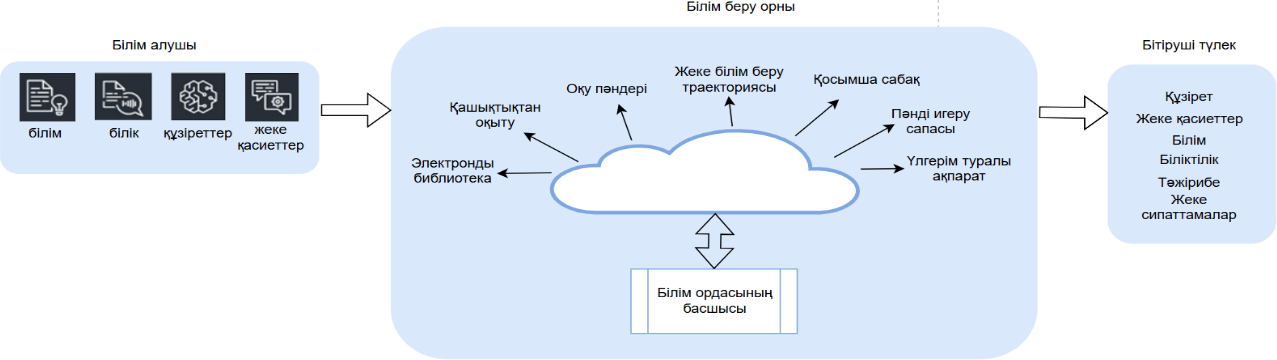
\includegraphics[width=0.8\textwidth]{media/ict/image99}
	\caption*{}
\end{figure}


{\bfseries 1-сурет. Білім беру процесінің жалпы моделі.}

Білім беру процесінің жалпы моделі -- білім беру процесінің әртүрлі
компоненттерінің ақпараттық технологияларды қолдану арқылы бір-бірінен
қалай әрекеттесеттінін сипаттайтын құрылым. Модель ақпараттық жүйелермен
бірге білім беру процесіне қатысушылар арасындағы оқыту, басқару және
өзара әрекеттесу процесін ұйымдастыруға және оңтайландыруға ықпал ету
көрінісін бейнелеп тұр.

Білім беруге негізделген ақпараттық жүйелерге қойылатын талаптар:

\begin{enumerate}
\def\labelenumi{\arabic{enumi}.}
\item
  Ақпаратты өңдеудің толықтығы -- қажетті ақпаратпен қажетті көлемде
  қамтамасыз ету.
\item
  Сапа -- жүйенің берілген функцияларды орындауға жарамдылық дәрежесі.
\item
  Ақпараттық жүйеге деген сенімділік -- техникалық құралдары мен
  бағдарламалық жасақтамасының арасында қателіктердің туындамауы.
\item
  Ақпараттық жүйенің қауіпсіздігі.
\item
  Пайдаланудың ыңғайлылығы -- әзірленетін жүйеде тиісті бөлімшенің
  ерекшеліктерін, онда өңделетін ақпарат пен әзірленетін құжаттардың
  құрамын, мазмұны мен нысандарын барынша есепке алуды талап ету.
\item
  Модульдік -- білім беруге арналған ақпараттық жүйенің элементтерін
  салыстырмалы түрде тәуелсіз және функционалды түрде аяқталған
  стандартты бөліктерден-модульдерден құру мүмкіндігі.
\item
  Сүйемелдеу -- сапаны жақсарту мүддесінде жүйенің ұзақ мерзімді
  пайдалануға және жетілдіруге жоғары дәрежеде бейімделуін қамтамасыз
  ету.
\end{enumerate}

Білім берудің заманауи ақпараттық жүйелері оқыту және оқу процесін
басқаруды айтарлықтай өзгертеді. Осы негізде білім беруге арналған
ақпараттық жүйені бірнеше категорияларға бөліп қарастырып, категорияға
сәйкес төмендегі 1-кестеде мысал ретінде бірнеше ақпараттық жүйелер
көрсетілген.

{\bfseries 1-кесте. Білім беру арналған ақпараттық жүйелер}

% \begin{longtable}[]{@{}
%   >{\raggedright\arraybackslash}p{(\columnwidth - 12\tabcolsep) * \real{0.1645}}
%   >{\raggedright\arraybackslash}p{(\columnwidth - 12\tabcolsep) * \real{0.0024}}
%   >{\raggedright\arraybackslash}p{(\columnwidth - 12\tabcolsep) * \real{0.0022}}
%   >{\raggedright\arraybackslash}p{(\columnwidth - 12\tabcolsep) * \real{0.4186}}
%   >{\raggedright\arraybackslash}p{(\columnwidth - 12\tabcolsep) * \real{0.0367}}
%   >{\raggedright\arraybackslash}p{(\columnwidth - 12\tabcolsep) * \real{0.0012}}
%   >{\raggedright\arraybackslash}p{(\columnwidth - 12\tabcolsep) * \real{0.3744}}@{}}
% \toprule\noalign{}
% \multicolumn{7}{@{}>{\raggedright\arraybackslash}p{(\columnwidth - 12\tabcolsep) * \real{1.0000} + 12\tabcolsep}@{}}{%
% \begin{minipage}[b]{\linewidth}\raggedright
% Оқытуды басқару жүйесі
% \end{minipage}} \\
% \midrule\noalign{}
% \endhead
% \bottomrule\noalign{}
% \endlastfoot
% \multicolumn{3}{@{}>{\raggedright\arraybackslash}p{(\columnwidth - 12\tabcolsep) * \real{0.1691} + 4\tabcolsep}}{%
% Атауы} & Артықшылығы &
% \multicolumn{3}{>{\raggedright\arraybackslash}p{(\columnwidth - 12\tabcolsep) * \real{0.4123} + 4\tabcolsep}@{}}{%
% Кемшілігі} \\
% \multicolumn{3}{@{}>{\raggedright\arraybackslash}p{(\columnwidth - 12\tabcolsep) * \real{0.1691} + 4\tabcolsep}}{%
% Moodlе} & Жаңа курс құру
% 
% Оқу процесін басқару
% 
% Мультимедиялық материалдар
% 
% Форумдар мен талқылаулар
% 
% Онлайн тестілеу
% 
% Оқушы үлгерімін бағалау &
% \multicolumn{3}{>{\raggedright\arraybackslash}p{(\columnwidth - 12\tabcolsep) * \real{0.4123} + 4\tabcolsep}@{}}{%
% Платформаны орнату қиындығы
% 
% Платформаны жаңарту кезіндегі қиындықтар
% 
% Пайдаланушы интерфейсі күрделі
% 
% Шектеулі интеграциялар
% 
% Техникалық қиындықтар} \\
% \multicolumn{3}{@{}>{\raggedright\arraybackslash}p{(\columnwidth - 12\tabcolsep) * \real{0.1691} + 4\tabcolsep}}{%
% Canvas} & Интуитивті интерфейс
% 
% Курстардың икемділігі
% 
% Бағалау және кері байланыс
% 
% Басқа платформалармен интеграция &
% \multicolumn{3}{>{\raggedright\arraybackslash}p{(\columnwidth - 12\tabcolsep) * \real{0.4123} + 4\tabcolsep}@{}}{%
% Орнатудың қиындылығы
% 
% Тегін нұсқаның шектеулі мүмкіндік-тері
% 
% Оқу уақыты} \\
% \multicolumn{7}{@{}>{\raggedright\arraybackslash}p{(\columnwidth - 12\tabcolsep) * \real{1.0000} + 12\tabcolsep}@{}}{%
% Онлайн оқыту платформасы} \\
% \multicolumn{3}{@{}>{\raggedright\arraybackslash}p{(\columnwidth - 12\tabcolsep) * \real{0.1691} + 4\tabcolsep}}{%
% Coursera} & Технологияның әртүрлі бағыттары бағыттары бойынша көпетеген
% курстар ұсынады
% 
% Белгілі университеттер мен компаниялардан сертификаттар мен дипломдар
% алу мүмкіндігі
% 
% Белсенді оқытуға ықпал ететін бейне жазбалар мен тесттер, тәжірибелік
% сабақтар &
% \multicolumn{3}{>{\raggedright\arraybackslash}p{(\columnwidth - 12\tabcolsep) * \real{0.4123} + 4\tabcolsep}@{}}{%
% Көптеген курстар ақылы
% 
% Сапалы және сапасыз курстардың санының көптігі
% 
% Оқытушылармен тарапынан жеткілікті қолдаудың болмағаны} \\
% \multicolumn{3}{@{}>{\raggedright\arraybackslash}p{(\columnwidth - 12\tabcolsep) * \real{0.1691} + 4\tabcolsep}}{%
% edX} & Беделді университеттердің курстары
% 
% Көптеген курстарды тегін оқу мүмкіндігі
% 
% MicroMasters және Professional Certificates
% 
% Іс жүзінде қолдануға мүмкіндік беретін тәжірибелік тапсырмалар &
% \multicolumn{3}{>{\raggedright\arraybackslash}p{(\columnwidth - 12\tabcolsep) * \real{0.4123} + 4\tabcolsep}@{}}{%
% Курстардың күрделілігі
% 
% Шектеулі интерактивті курстар
% 
% Платформадағы техникалық мәселелер} \\
% \multicolumn{7}{@{}>{\raggedright\arraybackslash}p{(\columnwidth - 12\tabcolsep) * \real{1.0000} + 12\tabcolsep}@{}}{%
% Бірлескен жұмыс құралдары} \\
% \multicolumn{2}{@{}>{\raggedright\arraybackslash}p{(\columnwidth - 12\tabcolsep) * \real{0.1668} + 2\tabcolsep}}{%
% Google workspace} &
% \multicolumn{4}{>{\raggedright\arraybackslash}p{(\columnwidth - 12\tabcolsep) * \real{0.4587} + 6\tabcolsep}}{%
% Gmail, Google Docs, Sheets, Slides, Drive жүйелермен бір уақытта жұмыс
% жасау мүмкіндігі
% 
% Бірнеше пайдаланушыға құжаттарды бір уақытта өңдеуге мүмкіндік беруі} &
% Интернетке тәуелділік
% 
% Деректердің құпиялылығы
% 
% Ақылы функцияларда мүмкіндіктер көптігі \\
% \multicolumn{2}{@{}>{\raggedright\arraybackslash}p{(\columnwidth - 12\tabcolsep) * \real{0.1668} + 2\tabcolsep}}{%
% Microsoft Teams} &
% \multicolumn{4}{>{\raggedright\arraybackslash}p{(\columnwidth - 12\tabcolsep) * \real{0.4587} + 6\tabcolsep}}{%
% Басқа Microsoft құралдарымен интегра­ция
% 
% Бірлескен мүмкіндіктер
% 
% Командалар мен сыныптарды басқару
% 
% Бейне конференциялармен сыныптарды басқару} & Платформаны орнатудың
% қиындығы
% 
% Тегін нұсқаның шектеулі мүмкіндік­тері
% 
% Пайдаланушы интерфейсінің күрделі­лігі
% 
% Деректерді қорғау және құпиялылық \\
% \multicolumn{7}{@{}>{\raggedright\arraybackslash}p{(\columnwidth - 12\tabcolsep) * \real{1.0000} + 12\tabcolsep}@{}}{%
% Виртуальды және толықтырылған шындық} \\
% Google Expeditions &
% \multicolumn{4}{>{\raggedright\arraybackslash}p{(\columnwidth - 12\tabcolsep) * \real{0.4599} + 6\tabcolsep}}{%
% Көптеген виртуальды турлармен экскурсияларға мүмкіндік
% 
% Интуитивтіинтерфейс
% 
% Мазмұнныңәртүрлілігі
% 
% виртуалдынысандарменөзараәрекеттесу мүміндігі} &
% \multicolumn{2}{>{\raggedright\arraybackslash}p{(\columnwidth - 12\tabcolsep) * \real{0.3756} + 2\tabcolsep}@{}}{%
% Жақсы интернет жүйесінің болуын қажет етеді
% 
% Виртуальды мүмкіндіктердің аздығы
% 
% Техникалық ақаулардың орын алу мүмкіндігі} \\
% zSpace &
% \multicolumn{4}{>{\raggedright\arraybackslash}p{(\columnwidth - 12\tabcolsep) * \real{0.4599} + 6\tabcolsep}}{%
% Тақырыптарды кеңінен түсінуге ықпал ететін виртуальды және толықтырылған
% шығдық тапсырмалары
% 
% Тақырыптардың кең ауқымы} &
% \multicolumn{2}{>{\raggedright\arraybackslash}p{(\columnwidth - 12\tabcolsep) * \real{0.3756} + 2\tabcolsep}@{}}{%
% Платформаның оқу орындары үшйн қымбаттылығы
% 
% Аппараттық және бағдарламалық жасақтаманы орнату қиындығы
% 
% Шектеулі қолжетімділік} \\
% \end{longtable}

Бұл технологиялар білім беруді жаңа мазмұнмен толтыру үшін, білім
алушылардың шығармашылығы мен шығармашылық қабілетін дамытатын оқытудың
жаңа формалары мен әдістерін қолдану үшін қолданылған кезде тиімді
болады.

Ашық білім беру жүйелерін дамыту білім беру мекемелерінің әлемдік білім
беру қызметтері нарығындағы бәсекелестігінің жаңа нысандарын тудырады.

Қазіргі білім саласы заманауи технологиялардың дамуымен, интернеттің
қолжетімділігінің арқасында айтарлықтар өзгерістерге ұшырауда. Білім
саласында қолданысқа ие платформалардың функциональдылығы барлық білім
алушыларға бір уақытта бірнеше адаммен байланыс орнатуға, ақпараттық
ресурстарға, конференциялар мен вебинарларға қатысуға, туындаған
мәселеге байланысты онлайн пікір таластырулар ұйымдастыруға мүмкіндік
береді (2-сурет).

\begin{figure}[H]
	\centering
	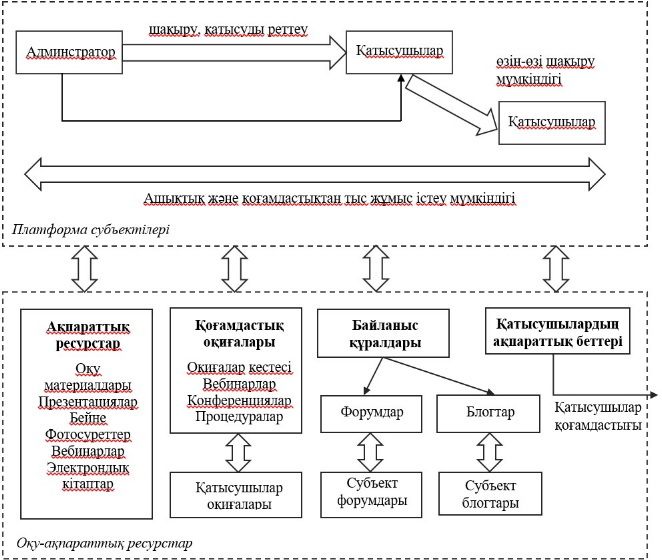
\includegraphics[width=0.8\textwidth]{media/ict/image100}
	\caption*{}
\end{figure}


{\bfseries 2-сурет. Білім беруге арналған ақпараттық жүйенің
фукнционалдылығы}

Ақпараттық жүйені әзірлеу білім беру процесін ұйымдастырудың заманауи
тәсілінің ерекшелігін көрсетеді, бұл білім алушының жаңа білімді өз
бетінше алу қабілетін қалыптастыруға және оларды болашақ кәсіби
қызметтің міндеттерін шешуге қолдануға дайын болуға бағытталған қол
жетімді интерактивті білім беру ортасын құруды қамтиды {[}8{]}. Бүгінгі
таңда білім берудің әртүрлі салаларына ақпараттық жүйелерді енгізу
кезінде келесі міндеттер орындалуы тиіс. Білім алушының интеллектуалды
тұлғасын дамыту, жеке тұлғаны ақпараттық қоғам жағдайында жайлы өмір
сүруге бейімдеу, ақпаратты қабылдау және өңдеу қабілеттерін дамыту,
әлеуметтік дағдыларды жетілдіру, сондай-ақ қойылған міндетті тез талдау
және оңтайлы шешім табу мүмкіндігі {[}9{]}.

Оқу-тәрбие процесін қарқындату. Бұл тұжырымдама білім алушының алған
білім сапасын жоғалтпай және оқу ұзақтығын өзгертпестен білім алушыға
берілетін ақпарат көлемін ұлғайтуды білдіреді. Заманауи технологияларға
бағдарланған және болашақта еңбек нарығында өзін сенімді сезінуге
қабілетті ақпараттық сауатты адамды дайындау {[}10{]}.

{\bfseries Нәтижелер мен талдау.}Зерттеу барысында білім беру мекемелері
үшін ақпараттық жүйелерді әзірлеуде қолданылатын ағымдағы
тенденцияларды, әдістер мен құралдарға талдау жүргізілді.

Білім беруге арналған ақпараттық жүйелер мынадай қызмет түрлерін жүзеге
асыру мүмкіндігін қамтамасыз етеді:

\begin{itemize}
\item
  білім беру процесін жоспарлайды;
\item
  білім беру процесінің барысын және білім беру бағдарламаларын игеру
  нәтижелерін белгілейді;
\item
  білім алушылар арасындағы өзара іс -- қимыл, оның ішінде-интернет
  желісі арқылы қашықтықтан оқытады;
\item
  білім беру қызметін басқару міндеттерін шешу үшін білім беру процесі
  барысында қалыптастырылатын деректерді пайдалану мүмкіндігін
  жоғарылатады;
\item
  білім алушылар интернет желісінің ақпараттық білім беру ресурстарына
  бақыланатын қолжетімділікті арттырады;
\item
  білім беру мекемесінің білім беру саласындағы басқаруды жүзеге
  асыратын органдармен, сондай-ақ басқа да білім беру мекемелерімен және
  ұйымдарымен өзара іс-қимылды жеңілдетеді.
\end{itemize}

Білім алушылар мен педагогтардың өзара байланысын визулизациялауға
көмектесу үшін ақпараттық жүйенің архитектурасы жобаланды. Төменде
3-суртетте көрсетілген.

\begin{figure}[H]
	\centering
	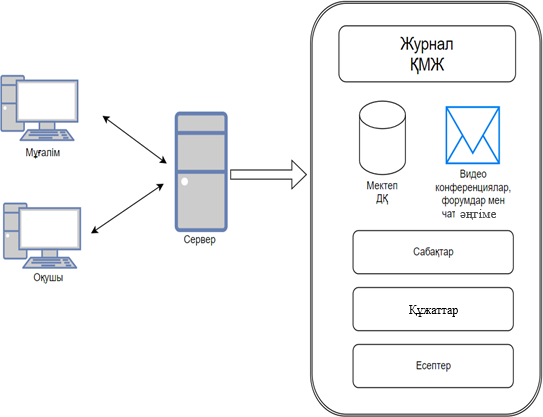
\includegraphics[width=0.8\textwidth]{media/ict/image101}
	\caption*{}
\end{figure}


{\bfseries 3-сурет. Ақпараттық жүйе архитектурасы}

Білім беруге арналған ақпараттық жүйенің архитектурасы білім беру
процесін қолдауға бағытталған компоненттердің құрылымдық сипаттамасы
және олардың өзара әрекеттесуі көруге көмектеседі (3-сурет). Ақпараттық
жүйенің әрбір бөлігін сипаттау үшін UML бірыңғай модельдеу тілі
қолданылды.

UML модельдеу тілі объектілерді, бизнес процестерді модельдеуге және
жүйелік жобалауға және ұйымдық құрылымдарды көрсетуге арналған
графикалық сипаттау тілі және ол бағдарламалаушыларға, жүйе
аналитиктеріне, дизайнерлерге жүйенің күрделі аспектілерін түсінуге
көмектеседі.UML тілінің басты мақсаты -- күрделі жүйелерді
визуализациялау және түсіну.

Білім беруге арналған ақпараттық жүйенің «Use case» диаграммасы --
ақпараттық жүйені жобалау процесінің бір бөлігі болып табылады және
жүйенің функционалдық талаптарын анықтау мен сипаттау үшін қолданылады.
Диаграмма -- ақпараттық жүйенің пайдаланушылармен қалай әрекеттесетінін
және оның қандай функцияларды орындайтынын көрсетеді (4-сурет).

\begin{figure}[H]
	\centering
	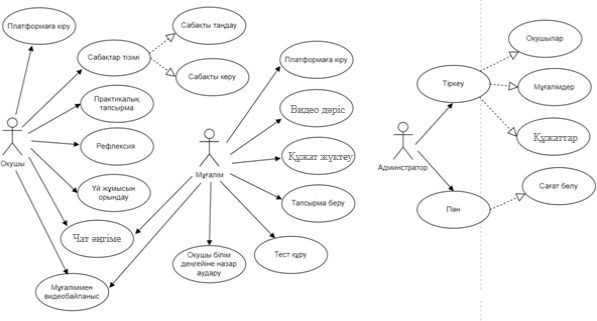
\includegraphics[width=0.8\textwidth]{media/ict/image102}
	\caption*{}
\end{figure}


{\bfseries 4-сурет. Use case диаграмма}

Ақпараттық жүйенің белгілі бір сценарий шеңберінде объектілер немесе
компоненттер арасындағы өзара әрекеттесуді визуализациялауға реттілік
диаграммасын қолдандық (5-сурет). Реттілік диаграммасы пайдаланушылар
мен ақпараттық жүйенің өзара байланысын қалыптастыруға негіз болды.

\begin{figure}[H]
	\centering
	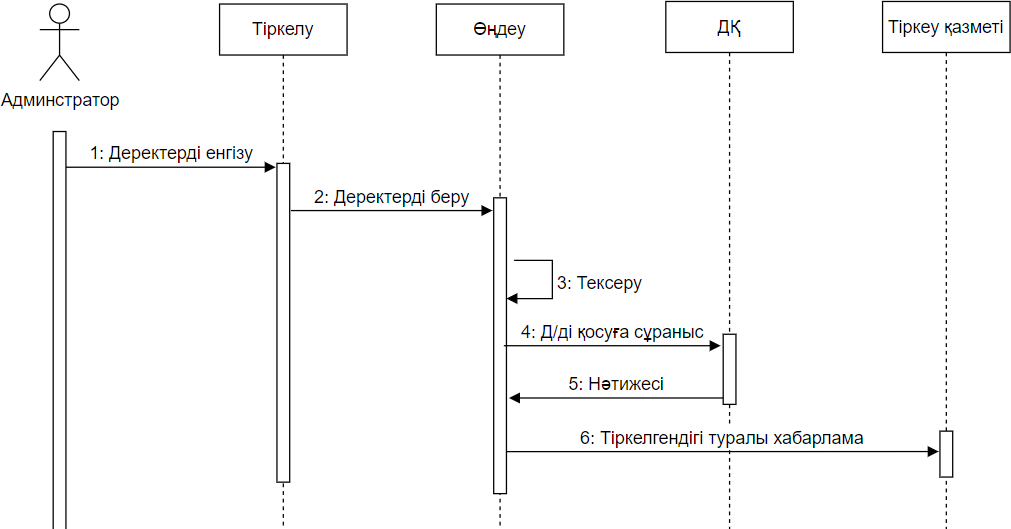
\includegraphics[width=0.8\textwidth]{media/ict/image103}
	\caption*{}
\end{figure}


{\bfseries 5-сурет. Ақпараттық жүйенің реттілік диаграммасы}

Диаграмма жүйенің компоненттері арасындағы әрекеттер мен хабарламалар
тізбегін көрсету арқылы пайдалану процестерін егжей-тегжейлі көрсетуге
көмектеседі. Бұл use case диаграммаларында анықталған функциялардың
қалай жүзеге асырылатынын жақсы түсінуге мүмкіндік береді.

Білім беруге арналған ақпараттық жүйе өте күрделі және көп уақытты талап
ететін процесс. Білім беру саласы дамып келе жатқандықтан көптеген
процестер жаңашылдықты, жаңа технологиялар мен жаңа ресурстарды талап
етеді.

{\bfseries Қорытынды.} Мақалада білім беруге арналған ақпараттық жүйені
әзірлеу мәселесі зерттелген және оның білім беру саласында заманауи
білім беру процесін ұйымдастыруға қажетті құрал екені дәлелденген.
Ақпараттық жүйелерді білім саласында сәтті енгізу білім алушылардың да,
педагогтардың да қажеттіліктерін қанағаттандырады және білім берудің
тиімділігі мен икемділігін едәуір арттыруға мүмкіндік береді.

Жобаланған ақпараттық жүйенің негізгі артықшылықтары:

\begin{enumerate}
\def\labelenumi{\arabic{enumi}.}
\item
  Оқытуды даралау. Жүйе білім алушының жеке қажеттіліктер мен
  қалауларына сәйкес материалды зерттеудің қарқыны мен дәйектілігін
  таңдай отырып, өздерінің білім беру траекториясын дербес құруға
  мүмкіндік береді.
\item
  Интерактивтілік және тәжірибелік фокус. Платформа білім алушылардың
  алған білімдері мен дағдыларын оқу процесінде белсенді қолдануға
  мүмкіндік беретін интерактивті жаттығулардың, тапсырмалардың және
  құралдардың кең ауқымын қамтиды.
\item
  Қашықтан және асинхронды өзара әрекеттесу. Білім алушылар теориялық
  материалды оқи алады, тапсырмаларды орындай алады және кезкелген
  педагогтан өздеріне ыңғайлы уақытта аудиториялық сабақтар шеңберімен
  шектелмей кері байланыс ала алады.
\item
  Үлгерім мониторингі және жеке қолдау. Жүйе білім алушылардың үлгерімін
  тиімді бақылауды, тапсырмаларды автоматтандырылған тексеруді және одан
  әрі оқыту бойынша жекелендірілген ұсыныстарды қамтамасыз етеді.
\end{enumerate}

Ақпараттық жүйені одан әрі жетілдіру оның функционалдық мүмкіндіктерін
кеңейтуге, басқа білім беру ресурстарымен интеграциялауға, сондай-ақ
әртүрлі оқу бағдарламалары мен білім беру ұйымдарының ерекшеліктеріне
бейімделуге бағытталуы мүмкін. Мұндай шешімдерді енгізу білім беруді
неғұрлым қолжетімді және тиімді етуге мүмкіндік береді.

{\bfseries Әдебиеттер}

\begin{enumerate}
\def\labelenumi{\arabic{enumi}.}
\item
  G.T.Balakayeva,D.K.Darkenbayev, M.Zhanuzakov.Development of a software
  system for predicting employee ratings // Informatyka, Autovatyka,
  Pomiary w Gospodarce I Pchronie Srodowiska, 2023. -- Vol.13(3). -P.
  121--124.DOI 10.35784/iapgos.3723
\item
  Ni Wayan Aprillia Pratiwi,Ida Bagus Surya Manuaba. The Effectiveness
  Of A Concrete Media Assisted Project Based Learning Model On Students
  ' Science Competency // Journal of Education
  Technology. -2020. -Vol.4(4). - P. 465-470.
  \href{https://doi.org/10.23887/jet.v4i4.27112}{DOI
  10.23887/jet.v4i4.27112}
\item
  Isa, W.A.R.W.M., Suhaimi, A.I.H., Noordin, N.~\emph{et al.} Hunger
  hero mobile application: applying soft system methodology at a local
  orphanage // International Journal of Information Technology. - 2023.
  -Vol.15, -P.691--696. DOI 10.1007/s41870-022-01101-w
\item
  Ade Mukhfir Guswara, Wawan Purwanto. The Contribution of Google
  Classroom Application and Motivation to The Learning Outcomes of Web
  Programming //Journal of Education Technology. -2020. -Vol.4(4). - P.
  424 - 432. \href{https://doi.org/10.23887/jet.v4i4.29896}{DOI
  10.23887/jet.v4i4.29896}
\item
  G.T.Balakayeva, P.Ezhichelvan, M.K.Tursynkozha. Analysis Research and
  Development of an Innovative Enterprise Digitalization System for
  Remote Work // International Journal of Mathematics and Physics.-2022.
  -Vol.13(1). -P.19-29.DOI 10.26577/ijmph.2022.v13.i1.02
\end{enumerate}

6.D.Darkenbayev. BigData processing on the example of credit scoring
//Journal of problems in computer science and information technologies.
- 2023. -Vol.1.-P.50 -- 61.

\href{https://doi.org/10.26577/1i32jpcsit2307}{DOI
10.26577/1i32jpcsit2307}

7.\href{https://link.springer.com/article/10.1007/s40593-024-00443-9\#auth-Yue-Huang-Aff1}{Yue
Huang},
\href{https://link.springer.com/article/10.1007/s40593-024-00443-9\#auth-Joshua-Wilson-Aff2}{Joshua
Wilson},
\href{https://link.springer.com/article/10.1007/s40593-024-00443-9\#auth-Henry-May-Aff2}{Henry
May}. Exploring the~Long‑Term Efects of~the~Statewide Implementation
of~an~Automated Writing Evaluation System on~Students' State Test ELA
Performance. // International Journal of Artifcial Intelligence in
Education. -2024. -Vol.34(3). -P. 1- 30. DOI 10.1007/s40593-024-00443-9

8.D.K.Darkenbayev, A.Altybay, Zh.Darkenbayeva, N.O.Mekebayev.
Intelligent Data Analysis on an Analytical platform // Informatyka,
Autovatyka, Pomiary w Gospodarce I Pchronie Srodowiska. - 2024.
-Vol.14(1). - P. 119-122. DOI 10.35784/iapgos.5423

9.Schwab M., Strobelt H., Tompkin J., Fredericks C., Huff C., Higgins
D., Strezhnev A., Komisarchik M., King, G., \&Pfister H. An Education
System with Hierarchical Concept Maps // IEEE Transactions on
Visualization and Computer Graphics.- 2016. -Vol.22(9). -P. 2111- 2124.
DOI 10.1109/TVCG.2016.2598518

10.\emph{S}hi, D., Cui W., Huang D., Zhang H., \& Cao N.
Reverse-Engineering Information Presentations: Recovering Hierarchical
Grouping from Layouts of Visual Elements // Association for Computing
Machinery. - 2022. -Vol.1(1). - P.1-21. DOI 10.1007/s44267-023-00010-1

\emph{{\bfseries Авторлар туралы мәліметтер}}

ДаркенбаевД.К. - PhD, әл-Фараби атындағы Қазақ ұлттық университетінің
доцент м.а., Алматы, Қазақстан, e-mail:
\href{mailto:dauren.kadyrovich@gmail.com}{\nolinkurl{dauren.kadyrovich@gmail.com}};

Жакшиликова Г.Ж. -Қазақ ұлттық қыздар педагогикалық университетінің
магистранты, Алматы, Қазақстан,e-mail: gulnur201801@gmail.com;

Мекебаев Н.О. - PhD, Қазақ ұлттық қыздар педагогикалық университетінің
қауымдастырылған профессор м.а., Алматы, Қазақстан, e-mail:
nurbapa@gmail.com

\emph{{\bfseries Information about the authors}}

D.Darkenbayev - PhD, Acting Associate Professor Al-Farabi Kazakh
National University,Almaty, Kazakhstan,e-mail:
\href{mailto:dauren.kadyrovich@gmail.com}{\nolinkurl{dauren.kadyrovich@gmail.com}};

G.Zhakshilikova - Master' s student, Kazakh National
Women' s Pedagogical University, Almaty,
Kazakhstan,e-mail: gulnur201801@gmail.com;

N.Mekebayev - PhD, Acting Associate Professor Kazakh National
Women' s Pedagogical University, Almaty,
Kazakhstan,e-mail:
\href{mailto:nurbapa@gmail.com}{\nolinkurl{nurbapa@gmail.com}}

ГРНТИ 28.23.39

{\bfseries APPLICATION OF AGGLOMERATIVE CLUSTERING FOR FORMING SKILL
COMMUNITIES OF JOB VACANCIES}

{\bfseries V. Ramazanova, M.Sambetbayeva, A}.{\bfseries Tokhmetov, Zh.
Lamasheva, S.Serikbayeva\textsuperscript{\envelope },}

\textsuperscript{1}L. N. Gumilyov Eurasian National University, Astana,
Kazakhstan,

{\bfseries \textsuperscript{\envelope }}Correspondent-author:
\href{mailto:inf_8585@mail.ru}{\nolinkurl{inf\_8585@mail.ru}}

One of the traditional methods for community detection in knowledge
graphs is agglomerative clustering. Agglomerative hierarchical
clustering is a widely used type of hierarchical clustering for grouping
objects based on their similarity. This method follows a bottom-up
approach, beginning with each individual data point considered as an
independent cluster, which are then continuously merged based on a
similarity threshold between clusters. This paper focuses on the use of
agglomerative clustering for analyzing skills extracted from job
postings on an online recruitment platform. It describes the approach to
data collection, processing, and subsequent clustering, providing an
overview of linkage methods between clusters and examples of the
application of various coefficients for quantitative assessment of
cluster quality. An analysis of bilingual clusters in Russian and
English is conducted, al-lowing for an evaluation of the versatility and
adaptability of the proposed approach to analyzing the multilingual
labor market in Kazakhstan. It was found that agglomerative clustering
methods hold significant potential for identi-fying structured groups of
skills, which can enhance the understanding of labor market trends and
needs. The analysis of clusters formed in different languages confirmed
the universality and adaptability of the proposed ap-proach to
multilingual data.

{\bfseries Keywords:} Sentence transformers, skills clustering,
agglomerative clustering, silhouette coefficient, skills communities.

{\bfseries ПРИМЕНЕНИЕ АГЛОМЕРАТИВНОЙ КЛАСТЕРИЗАЦИИ ДЛЯ ФОРМИРОВАНИЯ
СООБЩЕСТВ НАВЫКОВ ВАКАНСИЙ}

{\bfseries В.С.Рамазанова, М.А.Самбетбаева, А.Т. Тохметов, Ж.Б. Ламашева,
С.К.Серикбаева\textsuperscript{\envelope },}

\textsuperscript{1}Евразийский национальный университет им. Л. Н.
Гумилева, Астана, Казахстан,

e-mail:inf\_8585@mail.ru

Одним из традиционных методов обнаружения сообществ в графах знаний
является агломеративная кластеризация. Агломеративная иерархическая
кластеризация -- это широко используемый тип иерархической кластеризации
для группировки объектов на основе их сходства. Этот метод следует
подходу «снизу-вверх», начиная с того, что каждая отдельная точка данных
рассматривается как независимый кластер, которые затем непрерывно
объединяются на основе порога сходства между кластерами. В данной статье
основное внимание уделяется использованию агломеративной кластеризации
для анализа навыков, извлеченных из объявлений о вакансиях на
онлайн-платформе по подбору персонала. В ней описывается подход к сбору,
обработке и последующей кластеризации данных, дается обзор методов связи
между кластерами и примеры применения различных коэффициентов для
количественной оценки качества кластера. Проводится анализ двуязычных
кластеров на русском и английском языках, что позволяет оценить
универсальность и адаптивность предлагаемого подхода к анализу
многоязычного рынка труда в Казахстане. Было обнаружено, что методы
агломеративной кластеризации обладают значительным потенциалом для
выявления структурированных групп навыков, которые могут улучшить
понимание тенденций и потребностей рынка труда. Анализ кластеров,
сформированных на разных языках, подтвердил универсальность и
адаптивность предлагаемого подхода к многоязычным данным.

{\bfseries Ключевые слова:} Трансформеры предложений, кластеризация
навыков, агломеративная кластеризация, коэффициент силуэта, сообщества
навыков.

{\bfseries ЖҰМЫС ДАҒДЫЛАРЫ ҚАУЫМДАСТЫҒЫН ҚАЛЫПТАСТЫРУ ҮШІН АГЛОМЕРАТИВТІ
КЛАСТЕРЛЕУДІ ҚОЛДАНУ}

{\bfseries В.С.Рамазанова, М.А.Самбетбаева, А.Т.Тохметов, Ж.Б. Ламашева,
С.К.Серикбаева\textsuperscript{\envelope },}

\textsuperscript{1}Л.Н.Гумилев атындағы Еуразия ұлттық университеті,
Астана, Қазақстан,

e-mail: inf\_8585@mail.ru

Білім графтарында қауымдастықты анықтаудың дәстүрлі әдістерінің бірі
агломеративті кластерлеу болып табылады. Агломеративті иерархиялық
кластерлеу объектілерді ұқсастығына қарай топтастыру үшін иерархиялық
кластерлеудің кеңінен қолданылатын түрі болып табылады. Бұл әдіс әрбір
жеке деректер нүктесін тәуелсіз кластер ретінде өңдеуден бастап,
төменнен жоғарыға қарай әрекет етеді, содан кейін олар кластерлер
арасындағы ұқсастық шегіне негізделген үздіксіз біріктіріледі. Бұл жұмыс
онлайн жалдау платформасында жұмыс туралы хабарландырулардан алынған
дағдыларды талдау үшін агломеративті кластерлеуді пайдалануға
бағытталған. Ол деректерді жинау, өңдеу және кейіннен кластерлеу тәсілін
сипаттайды, кластерлер арасындағы байланыс әдістеріне шолу жасайды және
кластердің сапасын сандық бағалау үшін әртүрлі коэффициенттерді қолдану
мысалдарын береді. Орыс және ағылшын тілдеріндегі қостілді кластерлерге
талдау жүргізілді, бұл Қазақстанның көптілді еңбек нарығын талдауға
ұсынылып отырған тәсілдің әмбебаптығы мен бейімділігін бағалауға
мүмкіндік береді. Агломеративті кластерлеу әдістері еңбек нарығының
тенденциялары мен қажеттіліктерін түсінуді жақсартатын құрылымдық
дағдылар топтарын анықтау үшін маңызды әлеуетке ие екендігі анықталды.
Әртүрлі тілдерде қалыптасқан кластерлерді талдау көптілді деректерге
ұсынылған тәсілдің әмбебаптығы мен бейімделгіштігін растады.

{\bfseries Түйін сөздер:} Сөйлем трансформерлері, дағдыларды кластерлеу,
агломеративті кластерлеу, силуэт коэффициенті, дағдылар қауымдастықтары.

{\bfseries Introduction.} The rapid growth in the volume of data on skills
and qualifications available through online employment platforms
represents a rich source of information on current and future labor
market trends. However, due to their volume and diversity, clustering
methods play a crucial role in structuring this information. In the
context of graphs, communities, also known as clusters or modules, are
groups of vertices that typically share common characteristics and/or
perform similar functions within the graph {[}1{]}.

One of the methods for community detection in graphs is hierarchical
clustering. Applying agglomerative clustering methods to skills can
reveal not only existing groups of similar skills but also uncover
communities within knowledge graphs. Understanding and analyzing the
structures of skill communities can significantly enhance career
development strategies by fostering closer integration between
educational and professional training and market needs.

The goal of this work is to create clusters that group semantically
similar skills, which, though they may be phrased differently, retain
the same overall meaning. The results of such clustering are intended to
form communities of nodes in knowledge graphs, allowing for a deeper
exploration of skill structures in the market.

This paper focuses on the use of agglomerative clustering for analyzing
skills extracted from job postings on the online recruitment platform
HeadHunter in Kazakhstan. It describes the approach to data collection,
processing, and subsequent clustering, providing an overview of
methodologies and examples of applying various metrics to assess cluster
quality. An analysis and comparison of clusters obtained with different
agglomerative clustering parameters for sets of phrases in Russian and
English were conducted, allowing for an evaluation of the versatility
and adaptability of the proposed approach to analyzing the modern labor
market.

{\bfseries Literature review.} Hierarchical clustering is highlighted as
one of the traditional methods for community detection in graph
structures in article {[}1{]}. Hierarchical clustering is widely used in
various fields such as social networks and biology. This method begins
with defining a measure of similarity between all pairs of vertices.
Agglomerative algorithms, which merge clusters based on similarity, do
not require a pre-specified number of clusters, which is an advantage.
However, the main drawback of agglomerative hierarchical clustering is
poor scalability.

Articles {[}2{]} and {[}3{]} provide a detailed overview of various
agglomerative hierarchical clustering methods, such as single linkage,
complete linkage, average linkage, and Ward' s method.
These methods are used to group objects based on their similarity, which
is applicable to the analysis of skills from job postings. As noted in
{[}3{]}, the choice of metric and linkage method significantly impacts
clustering results, necessitating a careful approach to parameter
tuning. This is particularly important for text data analysis, where
selecting an appropriate metric can substantially affect the quality of
clusters and, consequently, skill analysis. The algorithm proposed in
article {[}4{]} presents a distributed approach to agglomerative
clustering that can be efficiently scaled to handle billions of objects.
Article {[}5{]} introduces the concept of using the Ordered Weighted
Averaging (OWA) operator to modify traditional linkages in agglomerative
hierarchical clustering. This method is of interest for research aimed
at enhancing the flexibility and robustness of clustering algorithms.

The use of the silhouette coefficient to evaluate cluster quality, as
demonstrated in {[}6{]}, allows for assessing the degree of separation
of clusters and determining the optimal number of clusters. On the other
hand, studies {[}7{]} highlight the limitations of the silhouette
coefficient and the Calinski-Harabasz index, which can lead to
misinterpretation of clustering results. In such cases, an additional
expert review of the data may be helpful to improve understanding of the
internal structure of the clusters.

Article {[}8{]} describes in detail how proper text preprocessing, such
as sentence segmentation, tokenization, stop-word removal, and
lemmatization, can significantly improve the quality and accuracy of
machine learning algorithms. The study {[}9{]} examines sentence vector
representations based on Transformer models in combination with various
clustering methods. Article {[}10{]} discusses the semantic accuracy of
models. The authors compare four freely available pre-trained sentence
transformer models (all-MiniLM-L6-v2, all-MiniLM-L12-v2,
all-mpnet-base-v2, and all-distilroberta-v1) on a sample of 6,110
articles and select the most efficient model, all-mpnet-base-v2.

Article {[}11{]} addresses the complex task of clustering categorical
data in data analysis. The author proposes an algorithm for clustering
job vacancies based on required skills using hierarchical clustering and
the Girvan-Newman method to identify job clusters. Article {[}12{]}
explores the use of two popular data clustering methods: K-Means and
agglomerative clustering, on data related to seafarer certification
skills. The authors analyze the advantages of each approach, including
K-Means ability to quickly process large volumes of data and provide
clearly delineated clusters, while agglomerative clustering offers a
detailed, hierarchical view of the data, useful for understanding
complex structures of certification requirements. The study {[}13{]}
analyzes the performance of text data clustering using the TF-IDF
method, fuzzy K-means, and hierarchical agglomerative clustering on
datasets such as News 20, Reuters, and email collections. The results
show that hierarchical agglomerative clustering provides better
performance compared to fuzzy K-means, including lower entropy and
higher F-measure values, indicating clearer separation and consistency
of clusters.

Article {[}14{]} describes the use of the Hierarchical Dirichlet Process
(HDP) for clustering documents that define skills in an industrial
environment for large IT companies. The article {[}15{]} studies
thematic clustering using TF-IDF and K-Means methods in the field of
information technology. The articles {[}16-17{]} consider clustering of
vacancies based on skills.

Thus, the literature review emphasizes the importance of selecting the
appropriate clustering methods and metrics in data analysis. Studies
show that hierarchical agglomerative clustering offers its advantages
depending on data characteristics and analysis goals. Clustering
efficiency increases with the use of adapted metrics and methods, which
is crucial for achieving accuracy and validity of results. The
implementation of innovative approaches enhances the flexibility and
scalability of methods, which is critically important when working with
large volumes of data. Assessing cluster quality through silhouette
coefficients and other indices helps determine the optimal number of
clusters, ensuring clearer data separation and consistency.

{\bfseries Materials and methods.} \emph{Collection, processing and
preparation of data embeddings.}

The dataset on skills was downloaded from the online recruitment site
hh.kz in Russian and English using the provided API
(https://api.hh.ru/vacancies) and the Python programming language.
Skills from job vacancies were collected over two months, from February
1, 2024, to March 31, 2024, from 177 localities in Kazakhstan, covering
25 professions in the information technology sector: analyst, art
director, creative director, game designer, designer, artist, chief
information officer (CIO), product manager, programmer, developer,
development team lead, project manager, network engineer, system
administrator, system engineer, information security specialist,
technical support specialist, tester, chief technology officer (CTO),
technical writer, system analyst, business analyst, methodologist, BI
analyst, data analyst, head of analytics department, DevOps engineer,
product analyst, and data scientist. The number of vacancies amounted to
5248. The number of unique skills totaled 3047.Skill phrases were
treated as sentences.

Next, from the data set of vacancies and skills, a knowledge graph was
built in the neo4j graph DBMS. Let' s consider the
ontological model of the graph of skills and vacancies. The graph
includes a set of entity classes: E\textsubscript{Recruitment} =
\{Vacancy, Skill, Requirement, Responsibility\} and a set of
relationships: R\textsubscript{Recruitment} = \{REQUIRE,
HAS\_REQUIREMENT, HAS\_RESPONSIBILITY\}.

Figure 1 presents a subgraph centered on the node representing the
vacancy "Senior IT Project Specialist (Aksai)" and other related skills
and vacancies. This node is connected to other nodes representing
skills, requirements, and responsibilities that describe various aspects
of its role and qualifications.

\begin{figure}[H]
	\centering
	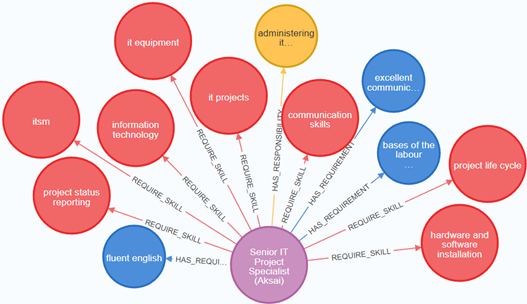
\includegraphics[width=0.8\textwidth]{media/ict/image104}
	\caption*{}
\end{figure}


{\bfseries Fig. 1. - Example of a subgraph of vacancies and skills. The
node representing the vacancy is marked in purple, skill nodes are
marked in red, requirement nodes are marked in blue, and responsibility
nodes are marked in yellow}

A notable feature of this graph is the presence of many paraphrased
skills that share the same meaning. Subsequently, it is necessary to
construct communities of semantically similar paraphrased skills for the
job vacancy skills graph.

Duplicates were removed from the set of skill phrases, all skills were
converted to lower case, and phrase embeddings were generated using the
paraphrase-multilingual-mpnet-base-v2 model.
Paraphrase-multilingual-mpnet-base-v2 is a pre-trained transformer model
designed to generate text embeddings, mapping sentences and paragraphs
into a 768-dimensional dense vector space. The model is trained on over
fifty languages and optimized to create vectors that effectively
represent the semantic content of text, making the embeddings
particularly useful for tasks related to paraphrase identification,
semantic search, and text clustering. The embeddings generated by this
model capture the semantic and contextual features of the text, making
them suitable for grouping texts by meaning.

\emph{Selection of clustering method, visualization and evaluation}.
Agglomerative clustering is a type of hierarchical clustering used to
group objects into clusters based on their similarity. It is considered
a "bottom-up" method because it starts with each object initially
considered as a separate cluster, and then, step by step, clusters are
merged until a specified number of clusters or a distance threshold is
reached (Fortunato, 2010).

The configuration for agglomerative clustering involves several
parameters: n\_clusters - the number of clusters to find, should be None
if distance\_threshold is specified; distance\_threshold - this
parameter sets the distance threshold to stop clustering; metric - a
``cosine'' or ``Euclidean'' metric was used to measure the distance
between clusters, if the relationship is ``ward'', only the "Euclidean"
metric is accepted; linkage - the link criterion determines what
distance to use between sets of observations. The algorithm will combine
pairs of clusters that minimize this criterion: ``ward'' minimizes the
variance of the clusters being merged, ``average'' uses the average of
the distances of each observation of two sets, ``full'' or ``maximum''
link uses the maximum distances between all observations of two sets,
``single'' uses the minimum distance between all observations of two
sets.

The visualization of the results was performed using the scikit-learn
and matplotlib libraries and the t-SNE (t-distributed Stochastic
Neighbor Embedding) dimensionality reduction technique (Scikit-learn
user guide, n.d.). The main advantage of t-SNE is its ability to
preserve local data structures, which makes it possible to identify
clusters and groups that may be hidden in high-dimensional data.

If the true cluster labels are unknown, clustering evaluation must be
performed using the model itself. The silhouette coefficient is an
example of such a score, where a higher silhouette coefficient score
refers to a model with more clearly defined clusters. Silhouette
coefficient is a metric that measures how well each data point fits into
its assigned cluster. It combines information about both the
connectivity (how close data point \emph{a} is to other points in its
own cluster) and separation (how far data point b is from points in
other clusters) of the data point technique (Scikit-learn user guide,
n.d.).

The Calinski-Harabasz index, also known as the Variance Ratio Criterion,
can also be used to evaluate the model, where a higher Calinski-Harabasz
score corresponds to a model with well-defined clusters. The score is
higher when clusters are dense and well-separated, which aligns with the
standard concept of a cluster technique (Scikit-learn user guide, n.d.).

Our approach to determining the optimal silhouette coefficient is based
on an iterative experimental programmatic process in which the distance
threshold between clusters was cyclically set for different proximity
metrics and linkage types to determine the maximum value of the
silhouette coefficient. Ranges of the «Distance\_threshold» parameter
were tested to determine the point at which a balance among the average
silhouette coefficient (should be maximum), the percentage of clusters
with negative silhouette coefficient (should be closer to zero), and
visual inspection of the clusters was observed. The program for the
cyclic process was implemented in Python using the Scikit-learn library.

{\bfseries Results and discussions.} As a result of the experiments, 3047
skill phrases were processed. Table 1 presents data on various metrics
(cosine, euclidean), linkage types (average, complete, single, ward),
distance threshold values, the number of clusters, the average
silhouette coefficient of all clusters, the percentage of clusters with
a silhouette coefficient above 0.03 (the most successful clusters), the
percentage of clusters with a negative silhouette coefficient, and the
average Calinski-Harabasz index.

The data for Table 1, starting from the fourth column, were obtained as
a result of cyclic operation of the agglomerative clustering algorithm
for three initial parameters (the first three columns), with
programmatically evaluation of cluster quality by silhouette and
Calinski-Harabasz coefficient algorithms.

{\bfseries Table 1 - Parameters and results of experiments}

% \begin{longtable}[]{@{}
%   >{\raggedright\arraybackslash}p{(\columnwidth - 14\tabcolsep) * \real{0.1062}}
%   >{\raggedright\arraybackslash}p{(\columnwidth - 14\tabcolsep) * \real{0.1074}}
%   >{\raggedright\arraybackslash}p{(\columnwidth - 14\tabcolsep) * \real{0.1198}}
%   >{\raggedright\arraybackslash}p{(\columnwidth - 14\tabcolsep) * \real{0.1198}}
%   >{\raggedright\arraybackslash}p{(\columnwidth - 14\tabcolsep) * \real{0.1358}}
%   >{\raggedright\arraybackslash}p{(\columnwidth - 14\tabcolsep) * \real{0.1470}}
%   >{\raggedright\arraybackslash}p{(\columnwidth - 14\tabcolsep) * \real{0.1322}}
%   >{\raggedright\arraybackslash}p{(\columnwidth - 14\tabcolsep) * \real{0.1317}}@{}}
% \toprule\noalign{}
% \multicolumn{3}{@{}>{\raggedright\arraybackslash}p{(\columnwidth - 14\tabcolsep) * \real{0.3334} + 4\tabcolsep}}{%
% \begin{minipage}[b]{\linewidth}\raggedright
% {\bfseries Clustering parameters}
% \end{minipage}} &
% \multirow{2}{=}{\begin{minipage}[b]{\linewidth}\raggedright
% {\bfseries Number of clusters}
% \end{minipage}} &
% \multirow{2}{=}{\begin{minipage}[b]{\linewidth}\raggedright
% {\bfseries Average silhouette coefficient of all clusters}
% \end{minipage}} &
% \multirow{2}{=}{\begin{minipage}[b]{\linewidth}\raggedright
% {\bfseries Percentage of clusters with silhouette coefficient greater than
% 0.03}
% \end{minipage}} &
% \multirow{2}{=}{\begin{minipage}[b]{\linewidth}\raggedright
% {\bfseries Percentage of clusters with negative silhouette coefficient}
% \end{minipage}} &
% \multirow{2}{=}{\begin{minipage}[b]{\linewidth}\raggedright
% {\bfseries Average Calinski-Harabasz index}
% \end{minipage}} \\
% \begin{minipage}[b]{\linewidth}\raggedright
% {\bfseries Metric}
% \end{minipage} & \begin{minipage}[b]{\linewidth}\raggedright
% {\bfseries Linkage}
% \end{minipage} & \begin{minipage}[b]{\linewidth}\raggedright
% {\bfseries Distance\_}
% 
% {\bfseries threshold}
% \end{minipage} \\
% \midrule\noalign{}
% \endhead
% \bottomrule\noalign{}
% \endlastfoot
% \multirow{23}{=}{cosine} & \multirow{12}{=}{average} & 0.2 & 1669 &
% 0.25506 & 33.97\% & 0\% & 9.60789 \\
% & & 0.24 & 1403 & 0.26764 & 40.77\% & 0.07\% & 9.03752 \\
% & & 0.25 & 1335 & 0.27106 & 42.77\% & 0.07\% & 9.03694 \\
% & & 0.26 & 1280 & 0.26711 & 43.44\% & 0.07\% & 8.88383 \\
% & & 0.27 & 1221 & 0.26728 & 44.31\% & 0\% & 8.83944 \\
% & & 0.28 & 1166 & 0.27018 & 46.14\% & 0\% & 8.77975 \\
% & & 0.29 & 1121 & 0.27126 & 47.55\% & 0\% & 8.76839 \\
% & & 0.3 & 1077 & 0.27041 & 48.75\% & 0.09\% & 8.76821 \\
% & & 0.31 & 1023 & 0.26873 & 49.76\% & 0.09\% & 8.74085 \\
% & & 0.32 & 978 & 0.26798 & 51.43\% & 0.1\% & 8.77425 \\
% & & 0.4 & 636 & 0.23460 & 61.16\% & 0.31\% & 8.96599 \\
% & & 0.5 & 357 & 0.17152 & 72.55\% & 0.84\% & 9.38007 \\
% & \multirow{8}{=}{complete} & 0.29 & 1342 & 0.28119 & 49.93\% & 2.6\% &
% 9.45677 \\
% & & 0.3 & 1295 & 0.28338 & 51.43\% & 2.78\% & 9.48204 \\
% & & 0.31 & 1257 & 0.28413 & 52.51\% & 2.86\% & 9.43280 \\
% & & 0.32 & 1222 & 0.28468 & 53.68\% & 2.86\% & 9.43222 \\
% & & 0.33 & 1175 & 0.28383 & 55.15\% & 2.89\% & 9.33287 \\
% & & 0.34 & 1143 & 0.28272 & 55.47\% & 3.32\% & 9.31358 \\
% & & 0.35 & 1099 & 0.28272 & 57.23\% & 3.37\% & 9.30610 \\
% & & 0.4 & 916 & 0.27294 & 63.54\% & 3 .93\% & 9.39409 \\
% & \multirow{3}{=}{single} & 0.2 & 1045 & -0.18031 & 19.14\% & 0.27\% &
% 2.39889 \\
% & & 0.29 & 406 & -0.28775 & 17.24\% & 0.49\% & 1.84882 \\
% & & 0.39 & 106 & -0.19031 & 17.92\% & 0.94\% & 1.89379 \\
% \multirow{3}{=}{euclidean} & \multirow{3}{=}{ward} & 2 & 1316 & 0.25526
% & 47.72\% & 4.79\% & 10.69402 \\
% & & 2.5 & 894 & 0.26155 & 62.08\% & 7.49\% & 10.48007 \\
% & & 2.9 & 666 & 0.24942 & 72.67\% & 9.46\% & 10.89370 \\
% \multicolumn{8}{@{}>{\raggedright\arraybackslash}p{(\columnwidth - 14\tabcolsep) * \real{1.0000} + 14\tabcolsep}@{}}{%
% {\bfseries Note
% -~\href{https://context.reverso.net/\%D0\%BF\%D0\%B5\%D1\%80\%D0\%B5\%D0\%B2\%D0\%BE\%D0\%B4/\%D0\%B0\%D0\%BD\%D0\%B3\%D0\%BB\%D0\%B8\%D0\%B9\%D1\%81\%D0\%BA\%D0\%B8\%D0\%B9-\%D1\%80\%D1\%83\%D1\%81\%D1\%81\%D0\%BA\%D0\%B8\%D0\%B9/Compiled+by+the+author}{Compiled
% by the author}}} \\
% \end{longtable}

When using cosine similarity with average linkage, a significant
reduction in the number of clusters from 1669 to 357 is observed as the
distance threshold increases from 0.2 to 0.5. In this parameter
configuration, the silhouette coefficient is of primary interest, and
the optimal threshold for balanced clustering is found to be between
0.28 and 0.3, where good silhouette scores are achieved while
maintaining a reasonable number of clusters.

For cosine similarity with complete linkage, the silhouette coefficient
varies from 0.28119 to 0.27294. The complete linkage method exhibits a
significant increase in the percentage of negative silhouettes (up to
3.93\% at a threshold of 0.4), which may be attributed to its tendency
to form clusters by combining distantly located elements, thereby
increasing group overlap.

When using cosine similarity with single linkage, poor clustering
quality is evident, with negative average silhouette values and low
Calinski-Harabasz index scores, indicating an unsuitable linkage method
for this type of data. The method exhibits negative average silhouette
values, indicating extremely weak separation between clusters.

For Euclidean similarity with Ward linkage, a threshold of 2.5 is
optimal in terms of the silhouette coefficient, providing a good balance
between the number and quality of clusters. The method shows an increase
in the percentage of negative silhouettes as the threshold increases,
reaching 9.46\% at a threshold of 2.9, indicating that as the threshold
increases, cluster quality deteriorates, and clusters become more
diffuse and overlapping.

The average and complete methods with cosine similarity generally yield
better silhouette coefficient results, particularly at intermediate
threshold values, allowing for a balance between the number of clusters
and their quality. The percentage of negative silhouette coefficients
indicates the degree of overlap or misclassification within groups,
serving as a crucial indicator of cluster structure quality. Further
examination of the data leads to the selection of cosine similarity with
average linkage and a distance threshold of 0.29, as this option
demonstrates the best silhouette coefficient results.

Figure 2 depicts the distribution of skill clusters using average
linkage with cosine similarity at a distance threshold of 0.29, where
each point represents a specific skill, and the color indicates
membership in one of the clusters.

\begin{figure}[H]
	\centering
	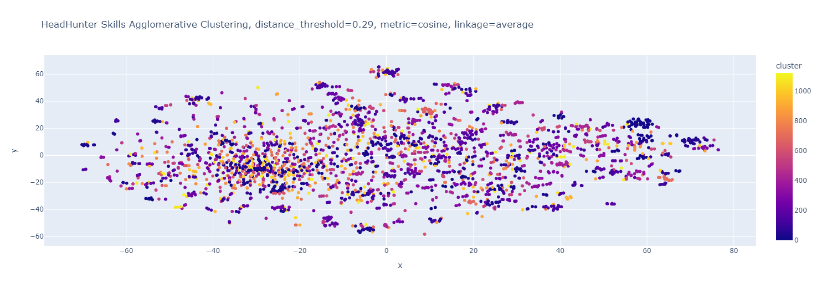
\includegraphics[width=0.8\textwidth]{media/ict/image105}
	\caption*{}
\end{figure}


{\bfseries Fig. 2 - Distribution of skill clusters using average linkage
with cosine similarity at a distance}

{\bfseries threshold of 0.29}

The points are evenly distributed across the graph, although there is
some concentration in the center. This may indicate common or frequently
occurring skills that do not exhibit distinct unique properties, in
contrast to rarer or more specialized skills found on the periphery.

Grouped points represent niche skills that are divided into several
clusters. For instance, Table 2 shows several clusters related to
testing. As described in the Materials and methods section, the
clustering data was collected in Russian and English. In this case, the
phrases in the data could be completely in the same language or contain
elements of both languages at the same time.

{\bfseries Table 2 - Example of clusters}

% \begin{longtable}[]{@{}
%   >{\raggedright\arraybackslash}p{(\columnwidth - 6\tabcolsep) * \real{0.1084}}
%   >{\raggedright\arraybackslash}p{(\columnwidth - 6\tabcolsep) * \real{0.7571}}
%   >{\raggedright\arraybackslash}p{(\columnwidth - 6\tabcolsep) * \real{0.1331}}
%   >{\raggedright\arraybackslash}p{(\columnwidth - 6\tabcolsep) * \real{0.0015}}@{}}
% \toprule\noalign{}
% \begin{minipage}[b]{\linewidth}\raggedright
% {\bfseries Cluster number}
% \end{minipage} & \begin{minipage}[b]{\linewidth}\raggedright
% {\bfseries Skills in the cluster}
% \end{minipage} & \begin{minipage}[b]{\linewidth}\raggedright
% {\bfseries Silhouette coefficient}
% \end{minipage} & \begin{minipage}[b]{\linewidth}\raggedright
% \end{minipage} \\
% \midrule\noalign{}
% \endhead
% \bottomrule\noalign{}
% \endlastfoot
% 248 & тестирование мобильного приложения, тестирование мобильных
% приложений, диагностика смартфонов & 0.53794 & \\
% 130 & автоматизированное тестирование, автотестирование, автоматизация
% тестирования, automation test, auto-testing & 0.5163 & \\
% 214 & тестирование пользовательского интерфейса, тестирование новых
% девайсов & 0.18981 & \\
% 478 & проведение ux/ui тестирований, unit testing, ui test & 0.1366 & \\
% 116 & test case, проведение тестирований, тестирование api,
% функциональное тестирование, нагрузочное тестирование, диагностика, a/b
% testing, ручное тестирование, тестирование, модульное тестирование,
% регрессионное тестирование, a/b тесты, диагностика пк, a/b тестирование,
% регресcионное тестирование, functional testing, кроссбраузерное
% тестирование, тестовая документация, тест-кейсы, testing framework,
% тест-дизайн, a/b-тестирование & 0.09042 & \\
% 976 & интеграционное тестирование & 0.0 & \\
% 1057 & beta-тестирования & 0.0 & \\
% 818 & тестирование qa & 0.0 & \\
% \multicolumn{4}{@{}>{\raggedright\arraybackslash}p{(\columnwidth - 6\tabcolsep) * \real{1.0000} + 6\tabcolsep}@{}}{%
% {\bfseries Note
% -~\href{https://context.reverso.net/\%D0\%BF\%D0\%B5\%D1\%80\%D0\%B5\%D0\%B2\%D0\%BE\%D0\%B4/\%D0\%B0\%D0\%BD\%D0\%B3\%D0\%BB\%D0\%B8\%D0\%B9\%D1\%81\%D0\%BA\%D0\%B8\%D0\%B9-\%D1\%80\%D1\%83\%D1\%81\%D1\%81\%D0\%BA\%D0\%B8\%D0\%B9/Compiled+by+the+author}{Compiled
% by the author}}} \\
% \end{longtable}

The list of clusters containing both Russian and English terms
highlights the bilingual nature of the data. Including skills in both
languages can enhance the understanding of professional competency
requirements across different regions, thereby increasing the
universality of research in employment and education.

Some clusters overlap with each other, which may result from fuzzy
boundaries between skills or the proximity of their content. Cluster 33
is the last cluster with a silhouette coefficient greater than zero.
Table 3 shows cluster 33, which includes many unrelated abbreviations
and monosyllabic terms.

{\bfseries Table 3 - Cluster 33}

% \begin{longtable}[]{@{}
%   >{\raggedright\arraybackslash}p{(\columnwidth - 6\tabcolsep) * \real{0.1083}}
%   >{\raggedright\arraybackslash}p{(\columnwidth - 6\tabcolsep) * \real{0.7564}}
%   >{\raggedright\arraybackslash}p{(\columnwidth - 6\tabcolsep) * \real{0.1329}}
%   >{\raggedright\arraybackslash}p{(\columnwidth - 6\tabcolsep) * \real{0.0025}}@{}}
% \toprule\noalign{}
% \begin{minipage}[b]{\linewidth}\raggedright
% {\bfseries Cluster number}
% \end{minipage} & \begin{minipage}[b]{\linewidth}\raggedright
% {\bfseries Skills in the cluster}
% \end{minipage} & \begin{minipage}[b]{\linewidth}\raggedright
% {\bfseries Silhouette coefficient}
% \end{minipage} & \begin{minipage}[b]{\linewidth}\raggedright
% \end{minipage} \\
% \midrule\noalign{}
% \endhead
% \bottomrule\noalign{}
% \endlastfoot
% 33 & java, верстка, vue, лвс, ui, vuejs, veam, sap fi, osi, скд, с\#,
% релиз, jpa, lte, асутп, сапр, asana, kotlin, впр, pestel, ge/m, vlan,
% java ee, сопровождение по, снип, itil, otrs, presales, nat, онбординг,
% sono, siem, unix, java se, idef, trello, глонасс, rtos, mbedos, срм,
% iis, koin di, vue js, pascal, kafka для очередей, fastapi, vuetify,
% фронтенд, удаленка, абис, uix, jest, nestjs, nodejs, цод, vrrp,
% айдентика, aiohtpp, парсер, сбор трейсов, zbrush, спецпроекты, ar, lld,
% асу тп, стпо, ai, impa, ррл, vite, бэм, плк, геттеры, смр, olap, aris,
% erspan, cacti, xunit, gradle, prd, gke, maven, ремонт п, пайка,
% переустановка по, trc, bem, сметы, гис, эсф, perco, vr, по, опс,
% java/kotlin, xamarin, лендинг, vtiger, биот, эдо, эквайринг, предовос,
% пэк, ппм, ндв, пдс, сзз, palo alto, jvm, суиб, волс, talend, пресейл,
% presale, pam, estaff, актуарий, uart, serdes, отладка, saml, элеткрик,
% пк, екв, в2в., wcdma & 0.0063 & \\
% \multicolumn{4}{@{}>{\raggedright\arraybackslash}p{(\columnwidth - 6\tabcolsep) * \real{1.0000} + 6\tabcolsep}@{}}{%
% {\bfseries Note
% -~\href{https://context.reverso.net/\%D0\%BF\%D0\%B5\%D1\%80\%D0\%B5\%D0\%B2\%D0\%BE\%D0\%B4/\%D0\%B0\%D0\%BD\%D0\%B3\%D0\%BB\%D0\%B8\%D0\%B9\%D1\%81\%D0\%BA\%D0\%B8\%D0\%B9-\%D1\%80\%D1\%83\%D1\%81\%D1\%81\%D0\%BA\%D0\%B8\%D0\%B9/Compiled+by+the+author}{Compiled
% by the author}}} \\
% \end{longtable}

An analysis of the table for Cluster 33 reveals a large number of
diverse skills, ranging from programming (Java, Kotlin, Node.js) to
specialized technical and engineering areas (soldering, repair, software
reinstallation). The very low silhouette coefficient (0.0063) indicates
that this cluster is poorly separated from others, possibly due to its
excessive heterogeneity.

The remaining skills do not form clusters and have a silhouette
coefficient of zero. These isolated skills constitute approximately 19\%
of the total number of skills.

Analyzing the results, it can be stated that the distribution of
silhouette coefficients reflects the quality of the clustering.
Typically, the silhouette coefficient ranges from 1 to -1. In our case,
clusters with a high silhouette coefficient, ranging from 1 to 0.04,
exhibit acceptable quality upon inspection and can be used to create
skill communities within a knowledge graph. Clusters with a silhouette
coefficient between 0.03 and 0 are not suitable for community creation
within the graph, as they have very blurred boundaries and include
overly heterogeneous terms. Clusters with a zero silhouette coefficient
include unique skills that do not cluster with other skill formulations.
Clusters with a negative silhouette coefficient are of very poor quality
and may include highly heterogeneous data. However, in our selected
configuration, such clusters were not observed as a result of the
experiments.

When the silhouette coefficient threshold for each cluster is set above
0.03, these clusters will subsequently be used to identify skill
communities within job and skill knowledge graphs.

In analyzing clusters formed from skills in both Russian and English, it
is important to note that this approach allows for the consideration of
linguistic diversity, making the clustering process more adaptive and
accurate for multilingual data. This approach enables a better
understanding of data structure and provides a higher-quality analysis
of skills or qualifications.

When analyzing potential clustering errors, a key pattern can be
observed that may affect cluster quality, particularly in relation to
phrase length. Short phrases or abbreviations often carry less unique
information and may be erroneously grouped due to similarities in
spelling or pronunciation. For example, abbreviations such as SCCM and
SCTP might be clustered with Scrum, despite differences in their
functions and applications.

For short words and abbreviations, it was necessary to improve embedding
generation algorithms and conduct additional clustering. The additional
training of the multilingual Paraphrase-multilingual-mpnet-base-v2 model
used for generating embeddings based on the paraphrase data set "short
abbreviation-full form" partially solved the problem.

Let' s consider the ratio of individual skills and
erroneous clusters with a positive silhouette coefficient obtained
before and after training. The correctness of cluster formation was
evaluated by an expert.

{\bfseries Table 4 - Comparison of erroneous clusters before and after
training the embedding model}

% \begin{longtable}[]{@{}
%   >{\raggedright\arraybackslash}p{(\columnwidth - 8\tabcolsep) * \real{0.1926}}
%   >{\raggedright\arraybackslash}p{(\columnwidth - 8\tabcolsep) * \real{0.1463}}
%   >{\raggedright\arraybackslash}p{(\columnwidth - 8\tabcolsep) * \real{0.2549}}
%   >{\raggedright\arraybackslash}p{(\columnwidth - 8\tabcolsep) * \real{0.2282}}
%   >{\raggedright\arraybackslash}p{(\columnwidth - 8\tabcolsep) * \real{0.1781}}@{}}
% \toprule\noalign{}
% \begin{minipage}[b]{\linewidth}\raggedright
% {\bfseries Embedding model}
% \end{minipage} & \begin{minipage}[b]{\linewidth}\raggedright
% {\bfseries Silhouette coefficient}
% \end{minipage} & \begin{minipage}[b]{\linewidth}\raggedright
% {\bfseries Number of clusters (including single terms)}
% \end{minipage} & \begin{minipage}[b]{\linewidth}\raggedright
% {\bfseries Percentage of Single Terms from Total Skills (3047)}
% \end{minipage} & \begin{minipage}[b]{\linewidth}\raggedright
% {\bfseries Percentage of erroneous clusters}
% \end{minipage} \\
% \midrule\noalign{}
% \endhead
% \bottomrule\noalign{}
% \endlastfoot
% Before training & 0,27126 & 1121 & 19,17\% & 19,74\% \\
% After training & 0,2851 & 1407 & 24\% & 13,97\% \\
% \end{longtable}

Fine-tuning the model led to an increase in the number of clusters,
which may indicate more detailed segmentation of skills. The increase in
the average silhouette coefficient and the percentage of successful
clusters points to improved clustering quality after fine-tuning the
model. The percentage of erroneous clusters decreased, further
confirming the model' s improved performance. After
further training, there was a partial improvement in results, but for
better results it is necessary to create a separate dictionary of
abbreviations.

To address the potential for scalability of our approach beyond the IT
sector, we can expand its applicability to other professional domains,
such as finance, healthcare, and engineering. The methodology can be
adapted to these areas by incorporating domain-specific skills.
Potential adaptations include the use of specialized embedding models
trained on sector-relevant text corpora, which would enable more
accurate clustering of context-specific skills. For instance, in the
healthcare sector, medical terminologies and technical jargon could be
incorporated into the embedding space to improve the identification of
skill communities. Similarly, in the finance sector, the inclusion of
financial industry terms and competencies could enhance the clustering
process.

{\bfseries Conclusions.} This study explored the application of
agglomerative hierarchical clustering for analyzing skills extracted
from an online recruitment platform. The research encompassed a broad
range of linkage methods and distance metrics, allowing for the
assessment and comparison of the effectiveness of each approach in the
context of clustering semantically diverse data.

It was found that agglomerative clustering methods hold significant
potential for identifying structured groups of skills, which can enhance
the understanding of labor market trends and needs. The analysis of
clusters formed in different languages confirmed the universality and
adaptability of the proposed approach to multilingual data.

However, certain issues were also identified during the analysis, such
as overlapping clusters and low silhouette coefficient values in some
clustering configurations. These observations have indicated the need
for further refinement of data preprocessing techniques to improve the
quality of results. After further training of the embedding model on
paraphrases, a partial improvement in results was observed, however, a
separate dictionary of abbreviations will be created for the best
results.

The findings of this study can be utilized to develop more effective
data analysis tools, including the creation of educational programs and
skill development strategies tailored to the evolving conditions of the
labor market. The proposed methods and approaches may also find
application in other areas where analyzing large volumes of textual
information is required to identify hidden patterns and relationships.

In conclusion, despite certain challenges, the results achieved confirm
the value and effectiveness of hierarchical agglomerative clustering as
a tool for deep data analysis, opening new avenues for further research
and practical applications in the field of data analytics.

\emph{{\bfseries Financing.} This research is funded by the Science
Committee of the Ministry of Science and Higher Education of the
Republic of Kazakhstan (Grant No. AP22783030).}

{\bfseries References}

\begin{enumerate}
\def\labelenumi{\arabic{enumi}.}
\item
  Fortunato, S. (2010). Community detection in graphs// Physics
  Reports.- 2010.-Vol.486(3-5).-P. 75-174.
  \href{https://doi.org/10.1016/j.physrep.2009.11.002}{DOI
  10.1016/j.physrep.2009.11.002}
\end{enumerate}

2. Oti, E., \& Olusola, M. (2024). Overview of agglomerative
hierarchical clustering methods //British Journal of Computer,
Networking and Information Technology.-2024.-Vol., 7(2).-P 14-23.
\href{https://doi.org/10.52589/BJCNIT-CV9POOGW}{DOI
10.52589/BJCNIT-CV9POOGW}

3.Tokuda, E. K., Comin, C. H., \& Costa, L. F. (2022). Revisiting
agglomerative clustering// Physica A: Statistical Mechanics and Its
Applications.- Vol.585, Article 126433.

DOI
\href{https://doi.org/10.1016/j.physa.2021.126433}{10.1016/j.physa.2021.126433}

\begin{enumerate}
\def\labelenumi{\arabic{enumi}.}
\setcounter{enumi}{1}
\item
  Sumengen, B. (2021). Scaling hierarchical agglomerative clustering to
  billion-sized datasets. arXiv, 2021. DOI
  \href{https://doi.org/10.48550/arXiv.2105.11653}{10.48550/arXiv.2105.11653}
\item
  Cena, A., \& Gagolewski, M. (2020). Genie+OWA: Robustifying
  hierarchical clustering with OWA-based linkages// Information
  Sciences.-2020.-Vol. 520.-P. 324-336.
\end{enumerate}

\href{https://doi.org/10.1016/j.ins.2020.02.025}{DOI
10.1016/j.ins.2020.02.025}

\begin{enumerate}
\def\labelenumi{\arabic{enumi}.}
\setcounter{enumi}{3}
\item
  Gagolewski, M., Bartoszuk, M., \& Cena, A. Are cluster validity
  measures (in)valid? //Information Sciences.-2021.-Vol. 581.- P.
  620-634. \href{https://doi.org/10.1016/j.ins.2021.10.004}{DOI
  10.1016/j.ins.2021.10.004}
\item
  Söküt Açar, T., \& Öz, N. A. The determination of optimal cluster
  number by silhouette index at clustering of the European Union member
  countries and candidate Turkey by waste indicators// Politeknik
  Dergisi.-2020.-Vol. 26(3).
  \href{https://doi.org/10.5505/pajes.2019.49932}{DOI
  10.5505/pajes.2019.49932}
\item
  TabassumA., Patil R. R. A survey on text pre-processing \& feature
  extraction techniques in natural language processing.//International
  Research Journal of Engineering and Technology.-2020ю-Vol.7(6).-
  P.4864-4867.
  \url{https://www.semanticscholar.org/paper/A-Survey-on-Text-Pre-Processing-\%26-Feature-in-Tabassum-Patil/f308488e996599115fe478c03b74a0b19b9a8f06}
\item
  Pugachev L., BurtsevM. (2021). Short text clustering with
  transformers, ArXiv:21.02.00541v1
\end{enumerate}

DOI
\href{http://dx.doi.org/10.28995/2075-7182-2021-20-571-577}{10.28995/2075-7182-2021-20-571-577}

\begin{enumerate}
\def\labelenumi{\arabic{enumi}.}
\setcounter{enumi}{7}
\item
  GalliC., Donos N.,CalciolariE. Performance of 4 pre-trained sentence
  transformer models in the semantic query of a systematic review
  dataset on peri-implantitis//Information.- 2024.- Vol.15(2), Article
  68. \href{https://doi.org/10.3390/info15020068}{DOI
  10.3390/info15020068}
\item
  Ternikov A. A. (2022). Skill-based clustering algorithm for online job
  advertisements// Izvestiya of Saratov University. Mathematics.
  Mechanics. Informatics.-2022.- Vol.22(2).-P. 250-265.
  \href{https://doi.org/10.18500/1816-9791-2022-22-2-250-265}{DOI
  10.18500/1816-9791-2022-22-2-250-265}
\item
  Karthikeyan, B. A comparative study on K-means clustering and
  agglomerative hierarchical clustering// International Journal of
  Emerging Trends in Engineering Researc.-2020.-Vol. 8(5).-P. 1600-1604.
  \href{https://doi.org/10.30534/ijeter/2020/20852020}{DOI
  10.30534/ijeter/2020/20852020}
\item
  Bafna, P., Pramod, D., \& Vaidya, A. (2016, March). Document
  clustering: TF-IDF approach. In 2016 International Conference on
  Electrical, Electronics, and Optimization Techniques (ICEEOT) (pp.
  61-66). \href{https://doi.org/10.1109/ICEEOT.2016.7754750}{DOI
  10.1109/ICEEOT.2016.7754750}
\item
  Srivastava, R., Hingmire, S., \& Palshikar, G. K. (2020). Clustering
  skills for industrial learning. TCS Research, Tata Research Design \&
  Development Centre, Hadapsar, Pune.
  \url{https://www.cse.msu.edu/~wangzh65/AI4EDU/papers/15.pdf}
\item
  Biloshchytskyi, A., Shamgunova, . M. ., \& Biloshchytska , S. .
  (2024). Exploration of the thematic clustering and collaboration
  opportunities in Kazakhstani research//Scientific Journal of Astana IT
  University.-2024.-Vol. 17(17).-P.106-121.
  \href{https://doi.org/10.37943/17ALVR8114}{DOI 10.37943/17ALVR8114}
\item
  Ternikov, A. A. Skill-based clustering algorithm for online job
  advertisements// Izvestiya of Saratov University. Mathematics.
  Mechanics. Informatics,.-2022.- 22(2).-P. 250 - 265.
\end{enumerate}

\href{https://doi.org/10.18500/1816-9791-2022-22-2-250-265}{DOI
10.18500/1816-9791-2022-22-2-250-265}

15. Dikov M.E., Shirobokova S.N. O variante formalizacii zadachi
izvlechenija kljuchevyh navykov i klasternogo analiza vakansij pri
realizacii kompleksnogo instrumentarij cifrovoj proforientacii.//
Inzhenernyj vestnik Dona.-2024.- № 3.- S.1-10.{[}in Russian{]}

\url{https://cyberleninka.ru/article/n/o-variante-formalizatsii-zadachi-izvlecheniya-klyuchevyh-navykov-i-klasternogo-analiza-vakansiy-pri-realizatsii-kompleksnogo}

\emph{{\bfseries Сведение об авторах}}

Рамазанова В. С.- магистр технических наук, Евразийский национальный
университет им. Л. Н. Гумилева, Астана, Казахстан, е-mail:
\href{mailto:ramazanovavs@gmail.com}{\nolinkurl{ramazanovavs@gmail.com}};

Самбетбаева М. А.- PhD, Евразийский национальный университет им. Л. Н.
Гумилева Астана, Казахстан,

е-mail:
\href{mailto:madina_jgtu@mail.ru}{\nolinkurl{madina\_jgtu@mail.ru}};

Тохметов А. Т. - доцент, Евразийский национальный университет им. Л.Н.
Гумилева, Астана, Казахстан, E-mail:
\href{mailto:attohmetov@mail.ru}{\nolinkurl{attohmetov@mail.ru}};

Ламашева Ж. Б. - PhD, Евразийский национальный университет им. Л. Н.
Гумилева, Астана, Казахстан,

е-mail:
\href{mailto:lamasheva_zhb@enu.kz}{\nolinkurl{lamasheva\_zhb@enu.kz}} ;

Серикбаева С. К. - PhD, Евразийский национальный университет им. Л. Н.
Гумилева, Астана, Казахстан,

е-mail: \href{mailto:inf_8585@mail.ru}{\nolinkurl{inf\_8585@mail.ru}}

\emph{{\bfseries Information about the authors}}

Ramazanova V. - master of technical sciences, L. N. Gumilyov Eurasian
National University, Astana, Kazakhstan, е-mail: ramazanovavs@gmail.com;

Sambetbayeva M. - PhD, L. N. Gumilyov Eurasian National University,
Astana, Kazakhstan, е-mail:
\href{mailto:madina_jgtu@mail.ru}{\nolinkurl{madina\_jgtu@mail.ru}};

Tokhmetov A. - associate professor, L.N. Gumilyov Eurasian National
University, Astana, Kazakhstan, е-mail:
\href{mailto:attohmetov@mail.ru}{\nolinkurl{attohmetov@mail.ru}};

Lamasheva Zh. - PhD, L.N. Gumilyov Eurasian National University, Astana,
Kazakhstan, е-mail:
\href{mailto:lamasheva_zhb@enu.kz}{\nolinkurl{lamasheva\_zhb@enu.kz}};

Serikbayeva S. - PhD, L.N. Gumilyov Eurasian National University,
Astana, Kazakhstan, е-mail:
\href{mailto:inf_8585@mail.ru}{\nolinkurl{inf\_8585@mail.ru}}